% !TeX root = RJwrapper.tex
\title{Explaining Predictions with Shapley Values---An Introduction to
the fastshap Package}
\author{by Brandon M. Greenwell and \ldots{}}

\maketitle

\abstract{%
An abstract of less than 150 words.
}

\hypertarget{todo}{%
\subsubsection{TODO:}\label{todo}}

\begin{itemize}
\tightlist
\item
  \sout{Flesh out outline/section headers.}
\item
  Finish bar tab example (or switch to something better).
\item
  Discuss SHAP as a unification of Shapley, LIME, etc.
\item
  Find a good place to talk about ``true to the model'' versus ``true to
  the data'': \url{https://arxiv.org/pdf/2006.16234.pdf} (I think this
  is important for motivating the SampleSHAP approximation, which relies
  on randomly permuting instance values.)
\item
  Fill out KernalSHAP section.
\item
  Find motivating example for \textbf{iml} package; maybe credit card
  default risk?
\item
  Find motivating example for \textbf{fastshap} package; maybe Ames
  housing?
\item
  Find motivating example of interfacing with \textbf{shap} via
  \textbf{reticulate}. Can probably lift from the \textbf{fastshap}
  vigenette here:
  \url{https://bgreenwell.github.io/fastshap/articles/fastshap-vs-shap.html}.
\end{itemize}

\hypertarget{introduction}{%
\subsection{Introduction}\label{introduction}}

Introductory section which may include references in parentheses
\citep{R}, or cite a reference such as \citet{R} in the text.

\hypertarget{background}{%
\subsection{Background}\label{background}}

So what's a Shapley value? The Shapley value is the average marginal
contribution of a \emph{player} across all possible \emph{coalitions} in
a \emph{game}. In the context of statistical/machines learning,

\begin{description}

  \item[Game:] The prediction task for a single observation $x$.
  
  \item[Gain:] The prediction for $x$ minus the average prediction for all training observations.
  
  \item[Players] The feature values of $x$ that collaborate to receive the gain (i.e., predict a certain value).
  
\end{description}

In particular, the Shapley contribution of the \(i\)-th feature to an
instance \(x\) is defined as \begin{equation}
\nonumber
\phi_i\left(x\right) = \frac{1}{p!} \sum_{\mathcal{O} \in \pi\left(p\right)} \left[\Delta Pre^i\left(\mathcal{O}\right) \cup \left\{i\right\} - Pre^i\left(\mathcal{O}\right)\right], \quad i = 1, 2, \dots, p,
\end{equation} where \ldots{}

A simple example may help clarify the main ideas.

\hypertarget{fairly-splitting-a-bar-tab}{%
\subsubsection{Fairly splitting a bar
tab}\label{fairly-splitting-a-bar-tab}}

Alex, Brad, and Brandon decide to go out for drinks after work. They
shared a few pitchers of beer, but nobody payed attention to how much
each person drank. What's a fair way to split the tab? Suppose we knew
the follow information, perhaps based on historical data:

\begin{itemize}

  \item If Alex drank alone, he'd only pay \$10.
  
  \item If Brad drank alone, he'd only pay \$20.
  
  \item If Brandon drank alone, he'd only pay \$10.
  
  \item If Alex and Brad drank together, they'd only pay \$25.
  
  \item If Alex and Brandon drank together, they'd only pay \$15.
  
  \item If Brad and Brandon drank together, they'd only pay \$13.
  
  \item If Ales, Brad, and Brandon drank together, they'd only pay \$30.

\end{itemize}

\textbf{FIXME:} Finish later\ldots{}

\begin{table}[]
\centering
\begin{tabular}{@{}llll@{}}
\toprule
                      & \multicolumn{3}{l}{Marginal contribution} \\ \midrule
Permutation           & Alex        & Brad         & Brandon      \\ \midrule
Alex, Brad, Brandon   & \$10        & \$15         & \$5          \\ 
Alex, Brandon, Brad   & \$10        & \$15         & \$5          \\
Brad, Alex, Brandon   & \$5         & \$20         & \$5          \\
Brad, Brandon, Alex   & \$10        & \$20         & \$0          \\
Brandon, Alex, Brad   & \$5         & \$15         & \$10         \\
Brandon, Brad, Alex   & \$17        & \$3          & \$10         \\ \midrule
Shapley contribution: & \$9.50      & \$14.67      & \$5.83       \\ \bottomrule
\end{tabular}
\caption{Marginal contribution for each permutation of Alex, Brad, and Brandon (i.e., the order in which they arrive). The Shapley contribution is the average marginal contribution across all permutations. (Notice how each row sums to the total bill of \$30.)}
\end{table}

So the next time the bartender asks how you want to split the tab, whip
out a pencil and do the math!

\hypertarget{advantages}{%
\subsubsection{Advantages}\label{advantages}}

\hypertarget{disadvantages}{%
\subsubsection{Disadvantages}\label{disadvantages}}

\hypertarget{estimating-shapley-values-via-monte-carlo-simulation-sampleshap}{%
\subsection{Estimating Shapley values via Monte Carlo simulation:
SampleSHAP}\label{estimating-shapley-values-via-monte-carlo-simulation-sampleshap}}

A single estimate of the contribution of \(x_i\) to \(f\left(x\right)\)
is nothing the more than the difference between two predictions, where
each prediction is based on a sort of Frankenstein instance that' are's
constructed by swapping out values between the instance being explained
(\(x\)) and an instance selected at random from the training data. To
help stabilize the results, the procedure is repeated a large number,
say, \(R\), times, and the result averaged together.

\begin{algorithm}
\begin{enumerate}
  \item For $j = 1, 2, \dots, R$:
  \begin{enumerate}
    \item Select a random permutation $\mathcal{O}$ of the sequence $1, 2, \dots, p$.
    \item Select a random instance $w$ from the training instances $\boldsymbol{X}$.
    \item Construct two new instances as follows:
    \begin{itemize}
      \item $b_1 = x$, but all the features in $\mathcal{O}$ that appear after feature $x_i$ get their values swapped with the corresponding values in $w$.
      \item $b_2 = x$, but feature $x_j$, as well as all the features in $\mathcal{O}$ that appear after $x_j$, get their values swapped with the corresponding values in $w$.
    \end{itemize}
    \item $\phi_{ij}\left(x\right) = f\left(b_1\right) - f\left(b_2\right)$.
  \end{enumerate}
  \item $\phi_i\left(x\right) = \sum_{j = 1} ^ R \phi_{ij}\left(x\right) / R$.
\end{enumerate}
\caption{Approximating the $i$-th feature's contribution to $f\left(x\right)$. \label{alg:SampleSHAP}}
\end{algorithm}

If there are \(p\) features and \(m\) instanced to be explained, this
requires \(2 \times R \times p \times m\) predictions (or calls to a
scoring function). In practice, this can be quite computationally
demanding, especially since \(R\) needs to be large enough to produce
good approximations to each \(\phi_i\left(x\right)\). In practice, this
depends on the variance of each feature in the observed training data,
but typically \(R >= 50--100\) will suffice (\textbf{Need reference}).

SampleSHAP can be computationally prohibitive if you need to explain
large data sets. Fortunately, you often only need to explain a handful
of predictions, for example the most extreme predictions. However,
generating explanations for the entire training set, or a large enough
sample thereof, can be useful for generating aggregated model summaries,
like Shapley-based variable importance plots \textbf{FIXME: Add
reference}.

\hypertarget{special-cases}{%
\subsection{Special cases}\label{special-cases}}

The following sections discuss two special cases where exact Shapley
explanations can be computed efficiently: additive linear models, and
shallow trees and tree ensembles.

\hypertarget{linear-models-linearshap}{%
\subsubsection{Linear models:
LinearSHAP}\label{linear-models-linearshap}}

\textbf{FIXME:} I believe these results assume independence between
features. Need to check corresponding reference in
\url{https://arxiv.org/pdf/2006.16234.pdf}.

\textbf{FIXME:} Cite somewhere \cite{strumbelj-2014-explaining}.

First, lets discuss how a feature's value contributes to a prediction
\(f\left(X\right)\) in a simple (additive) linear model. That is, let's
assume for a moment that \(f\) takes the form \begin{equation}
\nonumber
  f\left(X\right) = \beta_0 + \beta_1 X_1 + \dots + \beta_p X_p
\end{equation}

Recall that the contribution of the \(i\)-th feature to the prediction
\(f\left(X\right)\) is the difference between \(f\left(X\right)\) and
the expected prediction if the \(i\)-th feature's value were not known:
\begin{equation}
\nonumber
\begin{split}
  \phi_i\left(X\right) &= \beta_0 + \dots + \beta_i X_i + \dots + \beta_p X_p \\ &\quad\quad - \left(\beta_0 + \dots + \beta_i \E\left(X_i\right) + \dots + \beta_p X_p\right) \\
  &= \beta_i \left(X_i - \E\left(X_i\right)\right)
\end{split},
\end{equation} where we estimate \(\E\left(X_i\right)\) with the
corresponding sample mean \(\bar{X}_i\). The quantity
\(\phi_i\left(X\right)\) is also referred to as the
\emph{situational importance of $X_i$} \citep{achen-1982-interpreting}.

\hypertarget{tree-based-models-treeshap}{%
\subsubsection{Tree-based models:
TreeSHAP}\label{tree-based-models-treeshap}}

\textbf{FIXME:} Need to find the right balance of details and complexity
here.

\hypertarget{kernal-based-approximate-shapley-values-kernelshap}{%
\subsubsection{Kernal-based approximate Shapley values:
KernelSHAP}\label{kernal-based-approximate-shapley-values-kernelshap}}

KernelSHAP \citep{lundberg-2017-KernelSHAP} uses a specially-weighted
local linear regression to estimate SHAP values for any model. Unlike
SampleSHAP\ldots{}

\hypertarget{shapley-values-in-r-and-other-lnaguages}{%
\subsection{Shapley values in R (and other
lnaguages)}\label{shapley-values-in-r-and-other-lnaguages}}

Probably the first, and most widely used implementation of Shapley
explanations is the Python \pkg{shap} library
\citep{lundberg-2017-KernelSHAP}, which provides a Python implementation
of SampleSHAP, KernelSHAP, TreeSHAP, and a few other model-specific
Shapley methods (e.g., DeepSHAP, which is provides approximate Shapley
values for deep learning models).

The \CRANpkg{iml} package \citep{R-iml} provides the \code{Shapley()}
function, which is a direct implementation of
Algorithm\textasciitilde{}\ref{alg:SampleSHAP}. It is written in
\CRANpkg{R6} \citep{R-R6}.

Package \CRANpkg{iBreakDown} implements a general approach to explaining
the predictions from supervised models, called \dfn{Break Down}
\citep{gosiewska-2019-iBreakDown}. SampleSHAP values can be computed as
a special case from random Break Down profiles; see
\code{iBreakDown::\code{shap()} for details}.

\CRANpkg{shapper} provides an R interface to the Python \pkg{shap}
library using \CRANpkg{reticulate} \citep{R-reticulate}; however, it
currently only supports KernelSHAP (\pkg{shap} itself supports
SampleSHAP, TreeSHAP, LinearSHAP, as well as various other
model-specific Shapley explanation methods).

I'm also aware of two experimental packages supporting Shapley
explanations that are not currently on CRAN: \pkg{shapr}
\citep{R-sellereite} and \pkg{shapFlex} \citep{R-shapFlex}. As
previously discussed, one drawback of traditional Shapley values is the
assumption of independent features (an assumption made by many IML
procedures, in fact). To that end, the \pkg{shapr} package implements
Shapley explanations that can account for the dependence between
features \citep{aas-2019-explaining}, resulting in significantly more
accurate approximations to the Shapley values. The package also includes
an implementation of KernelSHAP that's consistent with the \pkg{shap}
package for Python. The \pkg{shapFlex} package, short for Shapley
flexibility, provides approximate Shapley values that incorporate causal
constraints into the model's feature space, as described in
\citet{frye-2019-asymmetric}.

TreeSHAP has been directly incorporated into most implementations of
XGBoost \citep{chen-2016-xgboost} (including \CRANpkg{xgboost}
\citep{R-xgboost}), CatBoost \citep{eronika-2017-catboost}, and LightGBM
\citep{ke-2017-lightgbm}. Both \CRANpkg{fastshap} \citep{R-fastshap} and
\CRANpkg{SHAPforxgboost} \citep{R-SHAPforxgboost} provide an interface
to \pkg{xgboost}'s TreeSHAP implementation.

\CRANpkg{fastshap} provides an efficient implementation of SampleSHAP
and makes it a viable option for explaining the predictions from model's
where efficient model-specific Shapley methods do not exist or are not
yet implemented.

In Julia, there's \pkg{SampleSHAP.jl}, which is a lightweight port of
\pkg{fastshap}; \pkg{ShapML.jl}, which is another Julia implementation
of SampleSHAP; and \pkg{ShapleyValues.jl}, which hasn't been updated
since 2016.

The next two sections illustrate more in-depth use of the \pkg{iml} and
\pkg{fastshap} packages, respectively.

\hypertarget{imlshapley}{%
\subsubsection{\texorpdfstring{\texttt{iml::Shapley()}}{iml::Shapley()}}\label{imlshapley}}

\hypertarget{fastshapexplain}{%
\subsubsection{\texorpdfstring{\texttt{fastshap::explain()}}{fastshap::explain()}}\label{fastshapexplain}}

Like many post-hoc interpretation techniques (e.g., PDPs and ICE
curves), SampleSHAP can be made more efficient by generating all the
data up front, and scoring it only once (or twice, in the case of
SampleSHAP). For example, PDPs and ICE curves can be efficiently
constructed with only a single call to a scoring function by generating
all of the required data up front using a single cross-join operation
(which can be done rather efficiently in SQL or Spark). The scored data
can then be post-processed/aggregated and displayed as either a PDP or
set of ICE curves. An example using Spark with \CRANpkg{sparklyr}
\citet{R-sparklyr} can be found here:
\url{https://github.com/bgreenwell/pdp/issues/97}.

Fortunately, a similar trick can be exploited for SampleSHAP. Whether
explaining a single instance with a large value of Monte Carlo reps
(\(R\)), or explaining a large number of instances, the basic idea is to
generate all the required Frankenstein instances \(b_1\) and \(b_2\)
upfront, and stored in matrices \(\boldsymbol{B}_1\) and
\(\boldsymbol{B}_2\), respectively.

For example, suppose we wanted to estimate the contribution of \(x_i\)
for each of the \(N\) rows of the available training data
\(\boldsymbol{X}\) using a single Monte-Carlo repetition in
Algorithm\textasciitilde{}\ref{alg:SampleSHAP} (i.e.,
\(R = 1\))\footnote{The same idea also extends to explaining new instances.}.
To start, we can generate the \(N\) random instances at once and store
them in an \(N \times p\) matrix \(\boldsymbol{W}\). Rather generating
\(N\) random permutations \(\mathcal{O}\), and constructing \(b_1\) and
\(b_2\) one at a time, the \pkg{fastshap} package uses C++---via
\CRANpkg{Rcpp} \citep{R-Rcpp}---to efficiently generate an
\(N \times p\) logical matrix \(\boldsymbol{\mathcal{O}}\), where
\(\boldsymbol{\mathcal{O}}_{kl} = 1\) if feature \(x_l\) appears before
feature \(x_i\) in the \(k\)-th permutation, and \(0\) otherwise. This
logical matrix can then be used to logically subset \(\boldsymbol{X}\)
and \(\boldsymbol{W}\) to more efficiently construct
\(\boldsymbol{B}_1\) and \(\boldsymbol{B}_2\) in a single swoop. The
matrices (or data frames) can then be each scored once, and the
difference taken, to generate a single replication of
\(\phi_i\left(x\right)\) for each row of \(\boldsymbol{X}\).

Suppose instead we want to estimate the contribution of \(x_i\) for a
single instance \(x\), but using a large value of \(R\) for accuracy. We
could employ the same trick, but in this case \(\boldsymbol{X}\) would
refer to the \(R \times p\) matrix, where each row is a copy of the
instance \(x\).

\pkg{fastshap} also uses efficient exact methods for the special cases
described in Sections\ldots{}

\pkg{fastshap} is faster at computing Shapley values for a single
feature for a large number of instances (or a large value of \(R\) for a
single instance). But what about a large number of features?
Fortunately, Algorithm\textasciitilde{}\ref{alg:SampleSHAP} can be
trivially parallelized across features, and this is built into
\pkg{fastshap}.

\hypertarget{example-a-simple-benchmark-comparison}{%
\subsubsection{Example: A simple benchmark
comparison}\label{example-a-simple-benchmark-comparison}}

This section provides a brief example comparing various implementations
of Shapley values using \href{https://www.kaggle.com/c/titanic}{Kaggle's
Titanic: Machine Learning from Disaster competition}. While the true
focus of the competition is to use machine learning to create a model
that predicts which passengers survived the Titanic shipwreck, we'll
focus on explaining predictions from a simple logistic regression model.

To start, we'll load the data, which are conveniently available in the
\CRANpkg{titanic} package \citep{R-titanic}, and do a little bit of
cleaning.

\begin{Schunk}
\begin{Sinput}
# Read in the data and clean it up a bit
titanic <- titanic::titanic_train
features <- c(
  "Survived",  # passenger survival indicator
  "Pclass",    # passenger class
  "Sex",       # gender
  "Age",       # age
  "SibSp",     # number of siblings/spouses aboard
  "Parch",     # number of parents/children aboard
  "Fare",      # passenger fare
  "Embarked"   # port of embarkation
)
titanic <- titanic[, features]
titanic$Survived <- as.factor(titanic$Survived)
titanic <- na.omit(titanic)

# Data frame containing just the features
X <- subset(titanic, select = -Survived)
\end{Sinput}
\end{Schunk}

Next, we'll use the stats::glm() to fit a logistic regression model with
only main effects (i.e., no tw-way interactions, etc.).

\begin{Schunk}
\begin{Sinput}
fit <- glm(Survived ~ ., data = titanic, family = binomial)
\end{Sinput}
\end{Schunk}

Suppose we wanted to explain the predicted survival probability for a
new passenger named Jack
Dawson\footnote{Insipiration for this example was taken from \url{https://modeloriented.github.io/iBreakDown/articles/vignette_iBreakDown_titanic.html.}}:

\begin{Schunk}
\begin{Sinput}
jack.dawson <- data.frame(
  Pclass = 3,
  Sex = factor("male", levels = c("female", "male")),
  Age = 20,
  SibSp = 0,
  Parch = 0,
  Fare = 15,  # lower end of third-class ticket prices; technically, Jack won his ticket
  Embarked = factor("S", levels = c("", "C", "Q", "S"))
)
\end{Sinput}
\end{Schunk}

Our logistic regression model predicts that Jack's log-odds of survival
is

\begin{Schunk}
\begin{Sinput}
predict(fit, newdata = jack.dawson)
\end{Sinput}
\begin{Soutput}
#>         1 
#> -1.845561
\end{Soutput}
\end{Schunk}

Yikes, that's equivalent to estimated 13.64\% predicted probability of
survival! With a baseline (i.e., average) survival rate of 40.62\%, can
we explain why the model predicts Jack to be much lower?
Enter\ldots Shapley values.

There is a growing number of R packages that provide Shapley
explanations, the two most popular arguably being \pkg{iml} and
\pkg{iBreakDown}. In this example, we'll compare those with
\pkg{fastshap}.

To start, we need to define a few things (prediction wrapper, as well as
both \pkg{iml}- and \pkg{iBreakDown}-related helpers).

\begin{Schunk}
\begin{Sinput}
# Prediction wrapper to compute predicted probability of survive
pfun <- function(object, newdata) {
  predict(object, newdata = newdata)
}

# DALEX-based helper for iBreakDown
explainer <- DALEX::explain(fit, data = X, y = titanic$Survived,                                             predict_function = pfun, verbose = FALSE)

# Helper for iml
predictor <- iml::Predictor$new(fit, data = titanic, y = "Survived",
                                predict.fun = pfun)
\end{Sinput}
\end{Schunk}

Next, we call each implementation's Shapley-related function to compute
explanations for Jack's prediction using 100 Monte Carlo repetitions.

\begin{Schunk}
\begin{Sinput}
# Compute explanations
set.seed(1039)  # for reproducibility
ex1 <- iBreakDown::shap(explainer, B = 100, new_observation = jack.dawson)
ex2 <- iml::Shapley$new(predictor, x.interest = jack.dawson, sample.size = 100)
ex3 <- fastshap::explain(fit, X = X, pred_wrapper = pfun, nsim = 100,
                         newdata = jack.dawson)
\end{Sinput}
\end{Schunk}

Finally, we plot the resulting explanations. Note that both
\pkg{fastshap} and \pkg{iBreakDown} plot the feature contributions in
the original order, whereas \pkg{iml} plots them in descending order.

\begin{Schunk}
\begin{Sinput}
library(ggplot2)

# Set ggplot2 theme
theme_set(theme_bw())

# Plot results (see Figure XYZ)
p3 <- plot(ex1) + ggtitle("iBreakDown")
p2 <- plot(ex2) + ggtitle("iml")
p1 <- autoplot(ex3, type = "contribution") + ggtitle("fastshap")
gridExtra::grid.arrange(p1, p2, p3, nrow = 1)
\end{Sinput}
\begin{figure}[!htb]

{\centering 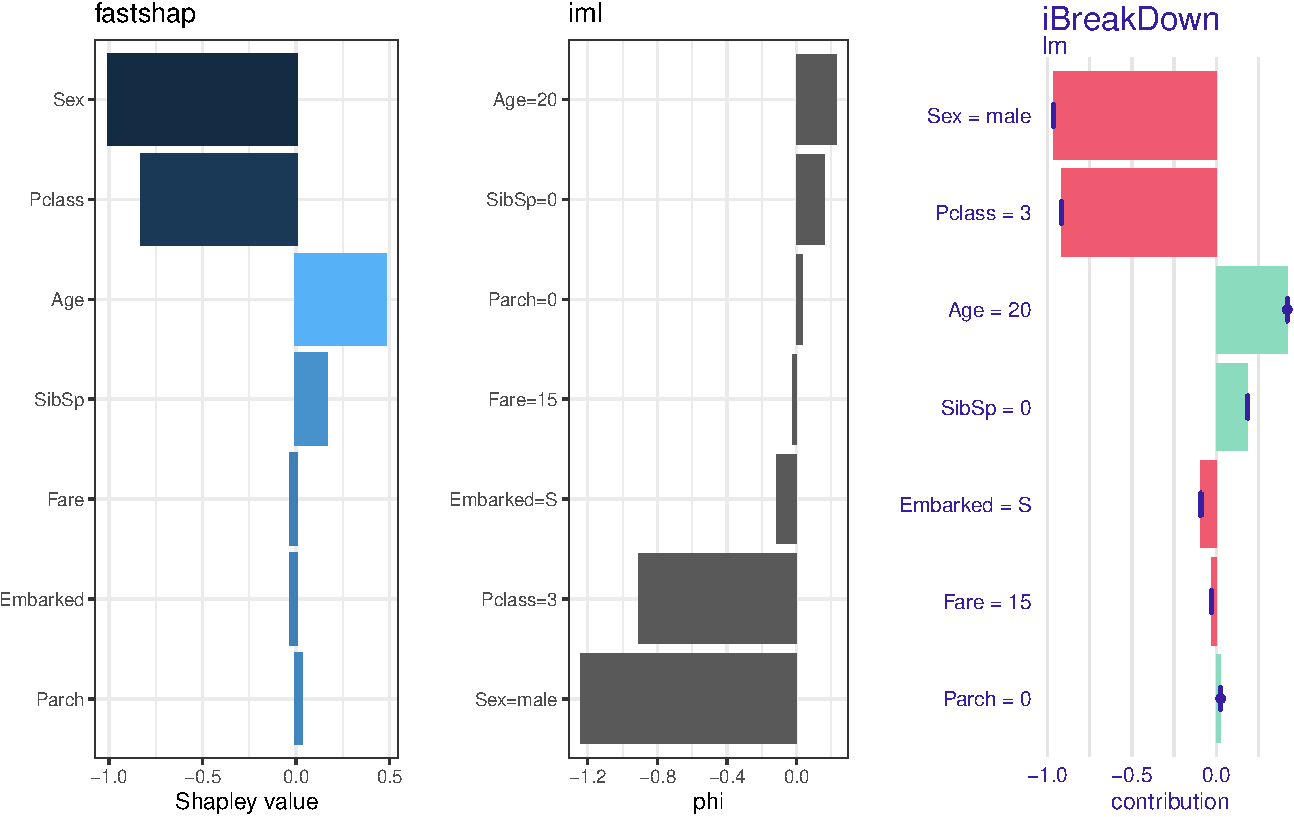
\includegraphics[width=1\linewidth]{greenwell_files/figure-latex/titanic-jack-explanations-plot-1} 

}

\caption[TBD]{TBD.}\label{fig:titanic-jack-explanations-plot}
\end{figure}
\end{Schunk}

Each package comes loaded with it's own bells and whistles (e.g.,
\pkg{iml} and \pkg{iBreakDown} have particularly fantastic
visualizations). The main selling point of \pkg{fastshap} is speed! For
example, all three packages (in fact, all general and practical
implementations of Shapley values) use
Algorithm\textasciitilde{}\ref{alg:SampleSHAP} which requires a large
number of Monte Carlo repetitions to achieve accurate results. Below is
a simple benchmark looking at the estimated time (in seconds) to explain
Jack's prediction as a function of the number of Monte Carlo repetitions
for each implementation. (Note that this comparison does not make use of
\pkg{fastshap}'s feature-wise parallelization.)

\begin{Schunk}
\begin{Sinput}
# Number of Monte Carlo reps for each simulation
nsims <- c(1, 5, 10, 25, 50, 75, seq(from = 100, to = 1000, by = 100))

# Initialize vectors to store timings
times1 <- times2 <- times3 <- numeric(length(nsims))

# Run simulation
set.seed(904)  # for reproducibility
for (i in seq_along(nsims)) {  # iBreakDown
  message("nsim = ", nsims[i], "...")
  times1[i] <- system.time({
    iBreakDown::shap(explainer, B = nsims[i], new_observation = jack.dawson)
  })["elapsed"]
  times2[i] <- system.time({  # iml
    iml::Shapley$new(predictor, x.interest = jack.dawson, 
                     sample.size = nsims[i])
  })["elapsed"]
  times3[i] <- system.time({  # fastshap
    fastshap::explain(fit, X = X, newdata = jack.dawson, pred_wrapper = pfun, 
                      nsim = nsims[i])
  })["elapsed"]
}

# Plot results
palette("Okabe-Ito")  # colorblind friendly palette 
plot(nsims, times1, type = "b", xlab = "Number of Monte Carlo repetitions",
     ylab = "Time (in seconds)", las = 1, pch = 19, 
     xlim = c(0, max(nsims)), ylim = c(0, max(times1, times2, times3)))
lines(nsims, times2, type = "b", pch = 19, col = 2)
lines(nsims, times3, type = "b", pch = 19, col = 3)
legend("topleft",
       legend = c("iBreakDown", "iml", "fastshap"),
       lty = 1, pch = 19, col = 1:3, inset = 0.02)
\end{Sinput}
\begin{figure}[!htb]

{\centering 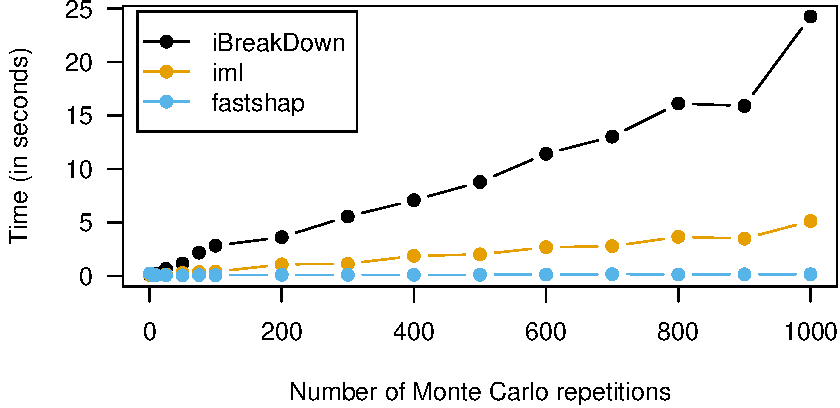
\includegraphics[width=1\linewidth]{greenwell_files/figure-latex/titanic-benchmark-1} 

}

\caption[Quick benchmark between three different implementations of SampleSHAP for explaining Jack's unfortunate prediction]{Quick benchmark between three different implementations of SampleSHAP for explaining Jack's unfortunate prediction.}\label{fig:titanic-benchmark}
\end{figure}
\begin{Sinput}
palette("default")  # switch back to R's default color palette
\end{Sinput}
\end{Schunk}

The message to be taken from
Figure\textasciitilde{}\ref{fig:titanic-benchmark} is that
\pkg{fastshap} scales incredibly well with \(N\) or \(R\), as long as
the corresponding \code{predict()} method does.

Oh, and \pkg{fastshap} can produce instant (and exact) Shapley
contributions for this example.

\begin{Schunk}
\begin{Sinput}
fastshap::explain(fit, newdata = jack.dawson, exact = TRUE)  # ExactSHAP
\end{Sinput}
\begin{Soutput}
#> # A tibble: 1 x 7
#>   Pclass    Sex   Age SibSp  Parch    Fare Embarked
#>    <dbl>  <dbl> <dbl> <dbl>  <dbl>   <dbl>    <dbl>
#> 1 -0.915 -0.964 0.420 0.186 0.0260 -0.0282  -0.0919
\end{Soutput}
\begin{Sinput}
fastshap::explain(fit, X = X, pred_wrapper = pfun, nsim = 10000,
                  newdata = jack.dawson)  # SampleSHAP
\end{Sinput}
\begin{Soutput}
#> # A tibble: 1 x 7
#>   Pclass    Sex   Age SibSp  Parch    Fare Embarked
#>    <dbl>  <dbl> <dbl> <dbl>  <dbl>   <dbl>    <dbl>
#> 1 -0.929 -0.977 0.422 0.185 0.0257 -0.0290  -0.0865
\end{Soutput}
\begin{Sinput}
predict(fit, newdata = jack.dawson, type = "terms")  # ExactSHAP (base R)
\end{Sinput}
\begin{Soutput}
#>       Pclass        Sex       Age     SibSp      Parch       Fare    Embarked
#> 1 -0.9153946 -0.9644851 0.4204564 0.1861824 0.02599872 -0.0281944 -0.09194646
#> attr(,"constant")
#> [1] -0.4781785
\end{Soutput}
\end{Schunk}

\textbf{FIXME:} Need a plot of fastshap explaining 1, 10, and 100 rows
for various values of \code{nsim} to show that the increase in
computation is not additive (i.e., it won't take twice as long to
epxlain two rows compared to just one, etc.)

\hypertarget{example-ames-housing-data}{%
\subsection{Example: Ames housing
data}\label{example-ames-housing-data}}

Use \texttt{fastshap::explain()} to explain predictions from a LightGBM
model on the Ames housing data using both exact and approximate
explanations (\textbf{Note:} there's a current PR that will give exact
functionality for LightGBM models, which is now on CRAN).

To start, we'll load the Ames housing data from the
\CRANpkg{AmesHousing} package \citep{R-AmesHousing} and fit a random
forest using the highly efficient \CRANpkg{ranger} \citep{R-ranger}
package.

\begin{Schunk}
\begin{Sinput}
library(ranger)

# Set ggplot2 theme
theme_set(theme_bw())

# Load Ames housing data
ames <- as.data.frame(AmesHousing::make_ames())

# Fit a (default) random forest
set.seed(1644)  # for reproducibility
(rfo <- ranger(Sale_Price ~ ., data = ames))
\end{Sinput}
\begin{Soutput}
#> Ranger result
#> 
#> Call:
#>  ranger(Sale_Price ~ ., data = ames) 
#> 
#> Type:                             Regression 
#> Number of trees:                  500 
#> Sample size:                      2930 
#> Number of independent variables:  80 
#> Mtry:                             8 
#> Target node size:                 5 
#> Variable importance mode:         none 
#> Splitrule:                        variance 
#> OOB prediction error (MSE):       623733174 
#> R squared (OOB):                  0.902265
\end{Soutput}
\end{Schunk}

Next we'll compute approximate Shapley values for the entire
\(2930 \times 80\) training set; to speed up computation, we'll turn on
parallel processing. (Note that this took about one hour on a 3.1 GHz
Dual-Core Intel Core i5 machine with 8 GB of RAM.)

\begin{Schunk}
\begin{Sinput}
library(doParallel)
library(fastshap)

# Set up parallel backend
cl <- if (.Platform$OS.type == "unix") 8 else makeCluster(8)
registerDoParallel(cl)

# Create data frame of only features
X <- subset(ames, select = -Sale_Price)

# Prediction wrapper
pfun <- function(object, newdata) {
  predict(object, data = newdata)$predictions
}

# Explain entire data set (useful for aggregated model summaries)
ex.all <- explain(rfo, X = X, nsim = 100, pred_wrapper = pfun, adjust = TRUE,
                  .parallel = TRUE)
head(ex)  # peak at results
\end{Sinput}
\end{Schunk}

\begin{Schunk}
\begin{Soutput}
#> # A tibble: 6 x 80
#>   MS_SubClass MS_Zoning Lot_Frontage Lot_Area Street Alley Lot_Shape
#>         <dbl>     <dbl>        <dbl>    <dbl>  <dbl> <dbl>     <dbl>
#> 1      284.       562.        2139.     6602.  0     -1.57      642.
#> 2     -308.        73.9        331.      346.  0      9.29     -282.
#> 3       -2.06     668.         977.     3331.  0     11.8       402.
#> 4      271.       729.        1603.     1313. -0.893 -4.70     -349.
#> 5      827.       437.         -67.2    2216.  0     -2.13      420.
#> 6      745.       812.          98.5     106.  0      4.41      369.
#> # ... with 73 more variables: Land_Contour <dbl>, Utilities <dbl>,
#> #   Lot_Config <dbl>, Land_Slope <dbl>, Neighborhood <dbl>, Condition_1 <dbl>,
#> #   Condition_2 <dbl>, Bldg_Type <dbl>, House_Style <dbl>, Overall_Qual <dbl>,
#> #   Overall_Cond <dbl>, Year_Built <dbl>, Year_Remod_Add <dbl>,
#> #   Roof_Style <dbl>, Roof_Matl <dbl>, Exterior_1st <dbl>, Exterior_2nd <dbl>,
#> #   Mas_Vnr_Type <dbl>, Mas_Vnr_Area <dbl>, Exter_Qual <dbl>, Exter_Cond <dbl>,
#> #   Foundation <dbl>, Bsmt_Qual <dbl>, Bsmt_Cond <dbl>, Bsmt_Exposure <dbl>,
#> #   BsmtFin_Type_1 <dbl>, BsmtFin_SF_1 <dbl>, BsmtFin_Type_2 <dbl>,
#> #   BsmtFin_SF_2 <dbl>, Bsmt_Unf_SF <dbl>, Total_Bsmt_SF <dbl>, Heating <dbl>,
#> #   Heating_QC <dbl>, Central_Air <dbl>, Electrical <dbl>, First_Flr_SF <dbl>,
#> #   Second_Flr_SF <dbl>, Low_Qual_Fin_SF <dbl>, Gr_Liv_Area <dbl>,
#> #   Bsmt_Full_Bath <dbl>, Bsmt_Half_Bath <dbl>, Full_Bath <dbl>,
#> #   Half_Bath <dbl>, Bedroom_AbvGr <dbl>, Kitchen_AbvGr <dbl>,
#> #   Kitchen_Qual <dbl>, TotRms_AbvGrd <dbl>, Functional <dbl>,
#> #   Fireplaces <dbl>, Fireplace_Qu <dbl>, Garage_Type <dbl>,
#> #   Garage_Finish <dbl>, Garage_Cars <dbl>, Garage_Area <dbl>,
#> #   Garage_Qual <dbl>, Garage_Cond <dbl>, Paved_Drive <dbl>,
#> #   Wood_Deck_SF <dbl>, Open_Porch_SF <dbl>, Enclosed_Porch <dbl>,
#> #   Three_season_porch <dbl>, Screen_Porch <dbl>, Pool_Area <dbl>,
#> #   Pool_QC <dbl>, Fence <dbl>, Misc_Feature <dbl>, Misc_Val <dbl>,
#> #   Mo_Sold <dbl>, Year_Sold <dbl>, Sale_Type <dbl>, Sale_Condition <dbl>,
#> #   Longitude <dbl>, Latitude <dbl>
\end{Soutput}
\end{Schunk}

\begin{Schunk}
\begin{Sinput}
library(ggplot2)

# Set ggplot2 theme
theme_set(theme_bw())

# Shapley summary plots (see Figure XYZ)
p1 <- autoplot(ex.all, num_features = 20)
p2 <- autoplot(ex.all, type = "dependence", feature = "Gr_Liv_Area", X = X,
               color_by = "Central_Air", alpha = 0.3) +
  scale_color_viridis_d(direction = -1) +  # cool colors
  theme(legend.position = c(0.7, 0.2), 
        legend.key = element_rect(colour = "transparent", fill = "white"))
gridExtra::grid.arrange(p1, p2, nrow = 1)
\end{Sinput}
\begin{figure}[!htb]

{\centering 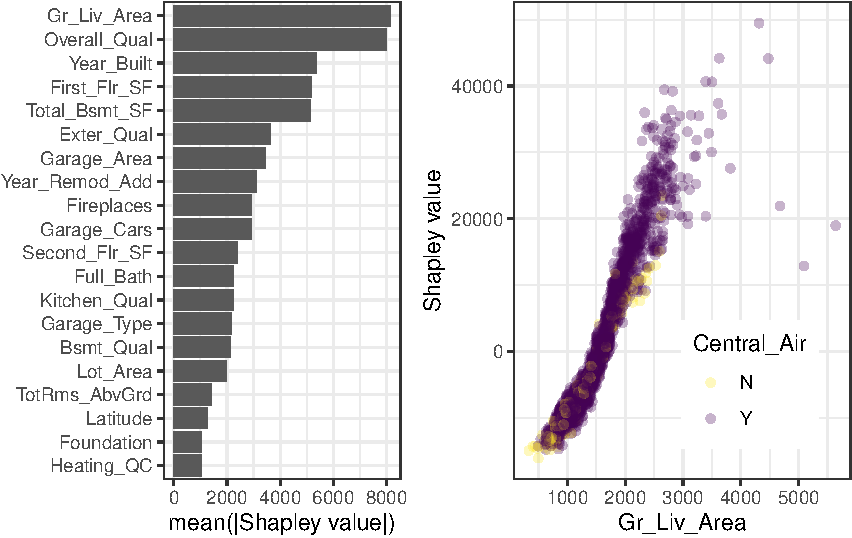
\includegraphics[width=1\linewidth]{greenwell_files/figure-latex/ex-ames-fastshap-autoplot-1} 

}

\caption[TBD]{TBD.}\label{fig:ex-ames-fastshap-autoplot}
\end{figure}
\end{Schunk}

\hypertarget{example-default-of-credit-card-clients}{%
\subsection{Example: default of credit card
clients}\label{example-default-of-credit-card-clients}}

Use \texttt{iml::Shapley()} to explain most extreme predictions.

\hypertarget{example-an-example-of-interfacing-directly-with-shap-via-reticulate-would-be-cool}{%
\subsection{Example: An example of interfacing directly with shap via
reticulate would be
cool!}\label{example-an-example-of-interfacing-directly-with-shap-via-reticulate-would-be-cool}}

TBD.

\hypertarget{summary}{%
\subsection{Summary}\label{summary}}

This file is only a basic article template. For full details of
\emph{The R Journal} style and information on how to prepare your
article for submission, see the
\href{https://journal.r-project.org/share/author-guide.pdf}{Instructions
for Authors}.

\bibliography{greenwell}


\address{%
Brandon M. Greenwell\\
University of Cincinnati\\%
2925 Campus Green Dr\\ Cincinnati, OH 45221\\ United States of
America\\ ORCiD---\href{https://orcid.org/0000-0002-8120-0084}{0000-0002-8120-0084}\\
%
%
%
\\\href{mailto:greenwell.brandon@gmail.com}{\nolinkurl{greenwell.brandon@gmail.com}}
}

\address{%
\ldots{}\\
University of Cincinnati\\%
2925 Campus Green Dr\\ Cincinnati, OH 45221\\ United States of
America\\ ORCiD---\href{https://orcid.org/0000-0002-8120-0084}{0000-0002-8120-0084}\\
%
%
%
\\\href{mailto:greenwell.brandon@gmail.com}{\nolinkurl{greenwell.brandon@gmail.com}}
}
